\section{\label{sec:method} Differentiable Adaptive Weighting}
\subsection{\label{sec:dds_motivation}Framework}

Commonly in machine learning, we seek to find parameters $\theta$ that minimize the \emph{risk} $J(\theta,P)$, the expected value of a loss function $\ell(x, y; \theta)$, where $\langle x, y \rangle$ are pairs of inputs and associated labels sampled from a particular distribution $P(X, Y)$:
\begin{equation}
  \label{eqn:generic_optim}
   \small
  \begin{aligned}
    \theta^* = \argmin_\theta J(\theta, P)
    ~~~\text{where}~~~
    J(\theta, P) = \mathbb{E}_{x, y \sim P(X, Y)} [\ell(x, y; \theta)]
  \end{aligned}
\end{equation}

In the ideal case, we would like the risk $J(\cdot)$ to be minimized over the inputs and outputs that we will expect our system to see at test time, defined as $P_{\text{test}}(X,Y)$.

To quantify the importance of training data, we propose to replace the distribution $\text{Uniform}(\mathcal{D}_\text{train})$, with a parameterized distribution $p(X, Y; \psi)$ with support of $\mathcal{D}_\text{train}$. In particular, data will be sampled by $\langle x, y \rangle \sim p(X, Y; \psi)$, 
and $\psi$ will be chosen so that $\theta^*$ that optimizes $J(\theta, p(X, Y;\psi))$ will approximately minimize $J(\theta, P_\text{dev}(X,Y))$: 
\begin{equation}
  \label{eqn:psi_theta_argmin}
   \small
  \begin{aligned}
    \psi^* = \argmin_\psi
    \sum_{i=1}^{N_\text{dev}} \ell(x_i, y_i; \theta^*(\psi))
    ~\text{where}~
    \theta^*(\psi) = \argmin_\theta \mathbb{E}_{x, y \sim p(X, Y; \psi)} \left[ \ell(x, y; \theta) \right]
  \end{aligned}
\end{equation}

Intuitively, $p(X, Y;\psi)$ is the optimal training data importance weight that adapts to the current model state $\theta$. Note that although the data importance weight is only parameterized by $\psi$, it is constantly optimized together with $\theta$ to provide an adaptive data usage ``guidance''. We name this formulation as Adaptive Importance Training. For the rest of the section, we abbreviate the training objective $J(\theta, p(X, Y;\psi))$ as $J(\theta, \psi)$ for ease of notation. Similarly, we abbreviate the risk $J(\theta, \text{Uniform}(\mathcal{D}))$ over a dataset $\mathcal{D}$ as $J(\theta, \mathcal{D})$.

\subsection{\label{sec:efficient_reward} Adaptive Weighting}
\begin{figure}
    \centering
    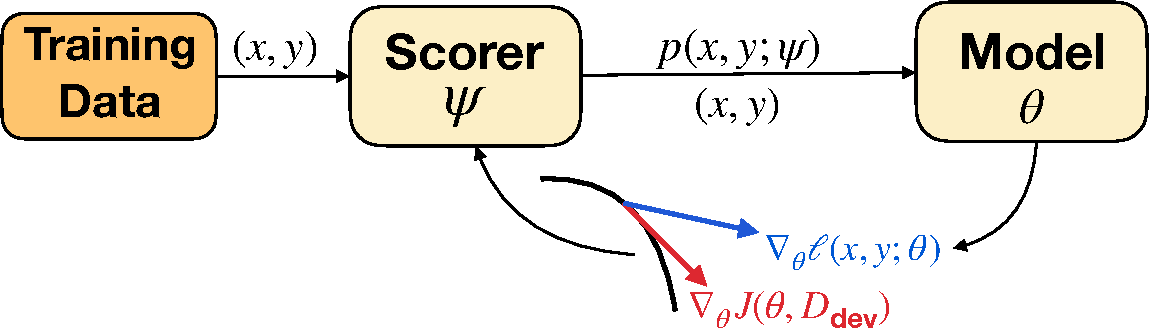
\includegraphics[width=0.5\textwidth]{figs/method_plot_crop.pdf}
    \caption{The general workflow of \dds.}
    \label{fig:method}
\end{figure}

In this section, we provide an intuitive explanation of how we update the model parameter $\theta$ and its adaptive weighting parameter $\psi$. Given the current optimal $\psi_t$ at time $t$, we can update $\theta$ as
\begin{align}
    \label{eqn:theta_update}
    \theta_t \leftarrow \theta_{t-1} + \alpha \nabla_\theta J(\theta_{t-1}, \psi_t)
\end{align}
where $\alpha$ is the learning rate for the model parameter $\theta$. The key problem left is, how can we optimize $\psi$ so that it provides the up-to-date data importance weights for the model $\theta_t$ at any time $t$ during training?

A straight-forward optimization strategy for $\psi$ is through Reinforcement Learning~(RL). Figure \ref{fig:method} illustrates the general framework of our method, where we can formulate the basic RL components as: the \textbf{agent} to optimize is the scorer, or data weighting function $P(x, y; \psi)$; the \textbf{state} is the current model parameter $\theta$; the \textbf{reward} $R(x, y)$ is the change in dev set risk $\Delta J_{\text{dev}}(x, y) = J(\theta_t, \mathcal{D}_\text{dev}) - J(\theta_{t-1}, \mathcal{D}_\text{dev})$, where $\theta_t$ is the new model parameter after updating $\theta_{t-1}$ using the training data $(x, y)$.

However, the above RL framework is difficult to implement in practice because of the drastic variance and credit assignment trade off in the reward function $\Delta J_{\text{dev}}(x, y)$: if we want to get clear credit assignment of a single training data pair $(x, y)$, its reward $\Delta J_{\text{dev}}(x, y)$ would be very noisy; to reduce the variance in $\Delta J_{\text{dev}}(x, y)$, we need a large number of training pairs $(x, y) = \{(x_0, y_0), (x_1, y_1), ..., (x_i, y_i)\}$. These examples would all get assigned the same amount of reward, while ideally they might have different level of influence on the final model performance.

To address this difficulty, we propose a novel reward function as an approximation to $\Delta J_{\text{dev}}(x, y)$ to quantify the effect of the training data $(x, y)$. In general, we prefer data that moves $\theta$ in the direction that minimizes the dev set risk. Therefore, we can use the agreement between the model gradient on data $(x, y)$ and the gradient on the dev set to approximate the \textit{change} in dev set risk brought by $(x, y)$. That is, 
\begin{align}
    \label{eqn:reward_fn}
    R(x, y) = \Delta J_{\text{dev}}(x, y) \approx \nabla_\theta \ell(x, y; \theta_{t-1}) \cdot \nabla_\theta J(\theta_t, \mathcal{D}_\text{dev}) 
\end{align}

According to the REINFORCE algorithm, the update rule for $\psi$ is thus
\begin{align}
    \label{eqn:psi_update}
    \psi_{t+1} \leftarrow  \psi_t + \eta \underbrace{\nabla_\theta \ell(x, y; \theta_{t-1}) \cdot \nabla_\theta J(\theta_t, \mathcal{D}_\text{dev})}_{\mathclap{R(x, y)}} \nabla_\psi \text{log}(P(X, Y;\psi))
\end{align}
where $\eta$ is the learning rate for the data importance parameter $\psi$. As shown in Figure \ref{fig:method}, by alternating between Eqn. \ref{eqn:theta_update} and Eqn. \ref{eqn:psi_update}, we can iteratively update $\theta$ using the adaptively weighted training data, and update $\psi$ to optimize data weighting for $\theta$. Now that we explain the intuition behind our method, we provide the mathematical derivation of the update rules in the next section.  

\subsection{\label{sec:diff_data_selection}Direct Differentiation}

The connection between $\psi$ and $\theta$ in Eqn. \ref{eqn:psi_theta_argmin} shows that $J(\theta_t, \mathcal{D}_\text{dev})$ is differentiable with respect to $\psi$. Notably, it is a specific case of bi-level optimization~\citep{bilevel_optim}, which has been applied to works on optimization~\citep{hyper_grad}, meta-learning~\citep{finn2017model}, and neural architecture search~\citep{darts}. To our knowledge, we are the first to utilize bi-level optimization for data selection. 

By the chain rule, we can compute the gradient $\nabla_\psi J(\theta_t, \mathcal{D}_\text{dev})$ as follows:
\begin{equation}
  \label{eqn:two_step_update}
   \small
  \begin{aligned}
    \nabla_\psi J(\theta_t, \mathcal{D}_\text{dev})
      &= \nabla_{\theta_t} J(\theta_t, \mathcal{D}_\text{dev})^\top \cdot \nabla_\psi \theta_t(\psi) &\text{(chain rule)} \\
      &= \nabla_{\theta_t} J(\theta_t, \mathcal{D}_\text{dev})^\top \cdot \nabla_\psi \left( \theta_{t-1} - \nabla_\theta J(\theta_{t-1}, \psi) \right) &\text{(substitute $\theta_t$ from Eqn~\ref{eqn:theta_update})} \\
      &\approx -\nabla_{\theta_t} J(\theta_t, \mathcal{D}_\text{dev})^\top \cdot \nabla_\psi  \left( \nabla_\theta J(\theta_{t-1}, \psi) \right) &\text{(assume $\nabla_\psi \theta_{t-1} \approx 0$)} \\
      &= \nabla_\psi \mathbb{E}_{x, y \sim p(X, Y; \psi)} \left[J(\theta_t, \mathcal{D}_\text{dev})^\top \cdot \nabla_\theta \ell(x, y; \theta_{t-1} )\right] \\
    &= \mathbb{E}_{x, y \sim p(X, Y; \psi)} \left[\left( J(\theta_t, \mathcal{D}_\text{dev})^\top \cdot \nabla_\theta \ell(x, y; \theta_{t-1} ) \right) \cdot \nabla_\psi \log{p(x, y; \psi)} \right]
  \end{aligned}
\end{equation}
Here, we make a Markov assumption that $\nabla_\psi \theta_{t-1} \approx 0$, assuming that at step $t$, given $\theta_{t-1}$ we do not care about how the values of $\psi$ from previous steps led to $\theta_{t-1}$. Eqn~\ref{eqn:two_step_update} leads to a rule to update $\psi$ using gradient descent:
\begin{equation}
  \label{eqn:psi_update_rule}
   \small
  \begin{aligned}
    \psi_{t+1} 
      &\leftarrow \psi_t + \eta \left( J(\theta_t, \mathcal{D}_\text{dev})^\top \cdot \nabla_\theta \ell(x, y; \theta_{t-1} ) \right) \cdot \nabla_\psi \log{p(x, y; \psi)},
  \end{aligned}
\end{equation}
where $\eta$ is the learning rate for $\psi$, which is a hyper-parameter. Now we can see that our derived update rule Eqn. \ref{eqn:psi_update_rule} matches the RL update rule according to our proposed reward function in Eqn. \ref{eqn:psi_update}. Since our formulation allows direct differentiation to optimize $\psi$, we name it Differentiable Adaptive Weighting~(\dds).

The connection between our design of the reward function and the direct derivation of the gradient of $\psi$ raises a potential concern with our approach: because we optimize $\psi_t$ directly on the dev set using $J(\theta_t, \mathcal{D}_\text{dev})$, we may risk indirectly overfitting model parameters $\theta_t$ by selecting a small subset of data that is overly specialized.
However we do not observe this problem in practice, and posit that this because (1) the influence of $\psi_t$ on the final model parameters $\theta_t$ is quite indirect, and acts as a ``bottleneck'' which has similarly proven useful for preventing overfitting in neural models \cite{grezl2007probabilistic}, and (2) because the actual implementations of DDS~(which we further discuss in Section \ref{sec:formualtion}) only samples a subset of data from $\mathcal{D}_\text{train}$ at each optimization step, further limiting expressivity.


\dds~operates by alternating Eqn~\ref{eqn:theta_update} and Eqn~\ref{eqn:psi_update} on batches of training data and dev data respectively. To implement Eqn~\ref{eqn:psi_update_rule} we need two approximations.
First, in practice the size of $\mathcal{D}_\text{train}$ is usually too large for exact calculation of the gradient $\nabla_\theta$. To overcome this difficulty, we adopt an importance sampling strategy, which can be implemented in two ways:
(1) We can sample a subset of $\mathcal{D}_{\text{train}}$ with a uniform proposal distribution $\hat{x}, \hat{y} \sim \text{Uniform}(\mathcal{D}_\text{train})$, then scale the probabilities in Eqn~\ref{eqn:psi_theta_argmin} by $p(\hat{x}, \hat{y}; \psi)$ over only this subset of data.
(2) We can similarly sample a subset of $\mathcal{D}_{\text{train}}$ uniformly, but then take a Monte-Carlo estimate of this quantity by further sub-sampling the data according to $p(\hat{x}, \hat{y}; \psi)$.
Second, the exact gradient for $\psi$ depends on the optimization algorithm that we use for $\theta$, and we discuss some concrete formulations in Appendix \ref{app:grad_of_optimizers}.